\documentclass[tikz,border=2pt]{standalone}
\usepackage{amsmath,amssymb}
\usepackage{pgfplots}
\pgfplotsset{compat=1.18}

\begin{document}
% The median m splits the distribution into two halves of probability 1/2 each; for the
% skewed density f(x) = x e^{-x} it lies at m = 1.678, left of the mean 2.
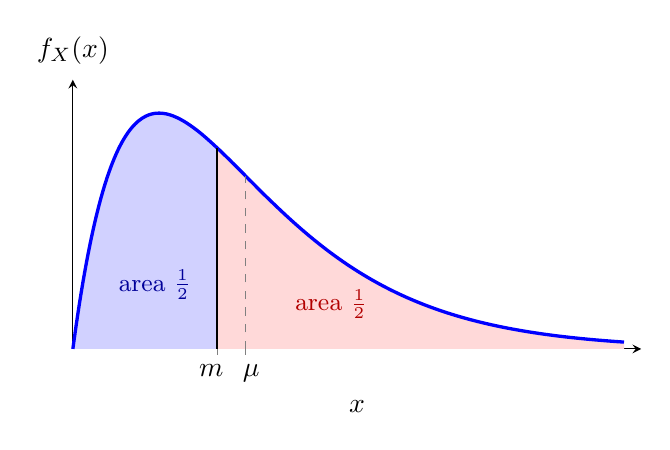
\begin{tikzpicture}
	\begin{axis}[
		axis lines=left, xmin=0, xmax=6.6, ymin=0, ymax=0.42,
		xtick={1.678,2}, xticklabels={$m\;\,$,$\;\,\mu$}, ytick=\empty,
		xlabel={$x$}, ylabel={$f_X(x)$}, ylabel style={rotate=-90, anchor=south, at={(axis description cs:0,1.02)}},
		samples=160, smooth, width=8.8cm, height=5cm, clip=false
		]
		\addplot[fill=blue!18, draw=none, domain=0:1.678] {x*exp(-x)} \closedcycle;
		\addplot[fill=red!15, draw=none, domain=1.678:6.4] {x*exp(-x)} \closedcycle;
		\addplot[blue, very thick, domain=0:6.4] {x*exp(-x)};
		\draw[black, thick] (axis cs:1.678,0) -- (axis cs:1.678,0.313);
		\node[blue!60!black, font=\small] at (axis cs:0.95,0.1) {area $\tfrac12$};
		\node[red!70!black, font=\small] at (axis cs:3.0,0.07) {area $\tfrac12$};
		\draw[gray, dashed] (axis cs:2,0) -- (axis cs:2,0.27);
	\end{axis}
	
\end{tikzpicture}
\end{document}
